\documentclass{article}
\usepackage[margin=0.75in]{geometry}
\usepackage{graphicx} 
\usepackage{natbib} 
\usepackage{amsmath} 

\setlength\parindent{0pt} % Removes all indentation from paragraphs
\addtolength{\topmargin}{-0.25in}
\usepackage[parfill]{parskip}
%\usepackage{times} % Uncomment to use the Times New Roman font

%----------------------------------------------------------------------------------------
%	DOCUMENT INFORMATION
%----------------------------------------------------------------------------------------

\title{Laboratory 5 : Builder}
%\author{Jacky Mallett}

\begin{document}

\maketitle % Insert the title, author and date

% If you wish to include an abstract, uncomment the lines below
% \begin{abstract}
% Abstract text
% \end{abstract}

%----------------------------------------------------------------------------------------
%	SECTION 1
%----------------------------------------------------------------------------------------

\section*{\centering Objectives}
In this laboratory you will explore the issues in building a very
simple economy, which uses debt to purchase objects. The goal
is to create a simulation where workers will continually build
and buy houses (each worker can buy a single house), using
loans.

The code for the experimental Builder Agent used in the simulation can be 
found in the file \emph{src/agent/Builder.java}. Note this code is
experimental.

The Builder Agent tries to build houses. It does this by taking a
construction loan
from a bank, and using that money to pay workers. There
are no materials involved, just labour costs. 

When the house is built it is listed on the House market for a price
above the builder's total loan costs. Workers in the simulation
can buy houses if the bank will grant them a loan. By default houses have
a TTL(Time to Live) of 120 months, which can be changed in the Builder.java
file. When this expires, the house is destroyed, and if the worker has
paid off their debt, they can attempt to buy another one.


\begin{enumerate}
\item Checks if sufficient workers are available to hire and that there are < 2 houses on the market
\item Tries to get a loan to build a house
\item If sucessful, hires workers, "builds" the house and lists on market
\item Fires all workers
\item Go to step 1
\end{enumerate}



\subsection*{Tips}
** Don't forget to save the simulation after you have created it, so that
you can reload it. **

How long is it reasonable to expect to run an artificial economy given the
frequency of financial crises in the real one?


% If you have more than one objective, uncomment the below:
%\begin{description}
%\item[First Objective] \hfill \\
%Objective 1 text
%\item[Second Objective] \hfill \\
%Objective 2 text
%\end{description}

%\subsection{Definitions}
%\label{definitions}
%\begin{description}
%\item[Stoichiometry]
%The relationship between the relative quantities of substances taking part in a reaction or forming a compound, typically a ratio of whole integers.
%\item[Atomic mass]
%The mass of an atom of a chemical element expressed in atomic mass units. It is approximately equivalent to the number of protons and neutrons in the atom (the mass number) or to the average number allowing for the relative abundances of different isotopes. 
%\end{description} 
 
%----------------------------------------------------------------------------------------
%	SECTION 2
%----------------------------------------------------------------------------------------

\section{Setup the Experiment}    
\begin{figure}[h]
\begin{center}
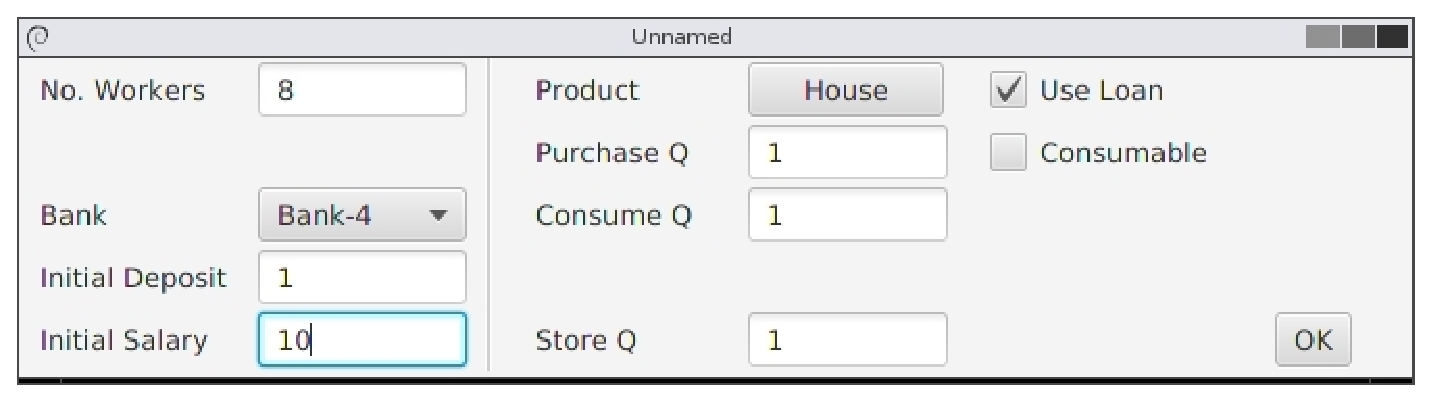
\includegraphics[width=12cm]{builderconfig.eps}
\caption{Configure Workers}
\end{center}
\end{figure}

\begin{enumerate}
\item Add a single Vanilla Bank to the Threadneedle simulation.
\item Add a single Builder (BR) to the simulation.
\item Add 10 Workers to the simulation, configure them as shown in
Figure \ref{fig:worker} Make sure you set the salary to 10
\item \emph{Save the simulation.}
\item Run the simulation.
\end{enumerate}

Click on the Builder Icon. The Output:Labour controls the amount
of labour required to build a single house in units of labour months. 
The builder will hire a maximum of 8 workers. 
\vspace{0.5cm}
How long will it take to build a house?

\vspace{0.5cm}
Why are house prices increasing? (Hint, look at the code.)

\vspace{0.5cm}
Why does the builder stop building?
\vspace{0.5cm}
How much are the workers getting paid?


\subsection*{Analysis}
Assume worker salaries are 1/month. By default the builder employs
8 workers.

How much does the builder list the first house for?

How much does a worker need to borrow in order to buy this house
as a multiple of their annual salary?
\section{Experiment 2}
Comment out the inflation line, "inflation += 1". 
\vspace{0.5cm}
How long does the simulation run?

\vspace{0.5cm}

Why does it stop?
\vspace{0.5cm}
\newpage
\section{Experiment 2: How long can the Agents keep building without crashing
the banking system?}
\begin{figure}[h]
\begin{center}
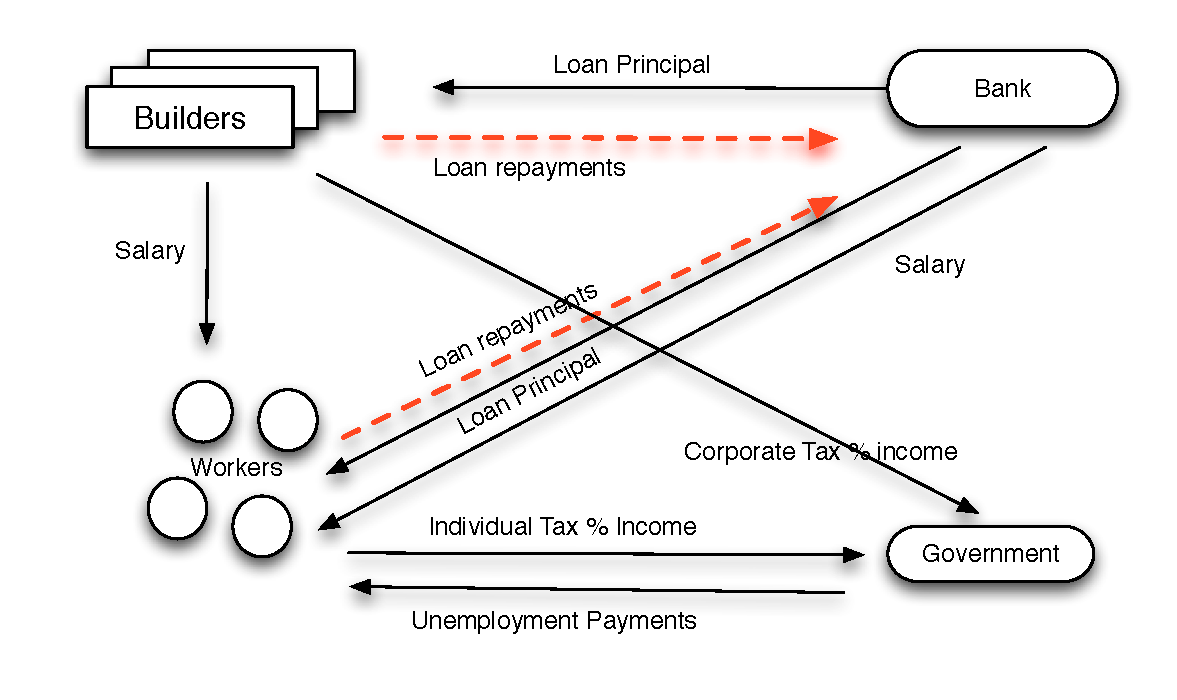
\includegraphics[width=12cm]{builder-exp.eps}
\caption{Configure Workers}
\end{center}
\end{figure}
Within the constraints of builders building houses and workers
buying them, you may have as many builders and workers as you
wish. Farms or other widget makers can also be modified. You can modify the Builder code, for example to have
different TTL's for the house, or to change profit calculation etc.

Keeping inflation turned off, create a steady state simulation
where builders build and workers borrow continuously. You will
need to adjust TTL and Labour:Output in order to ensure that houses
expire as soon as workers have finished paying them off. You may
have as many builders and workers as you like.

Now turn inflation back on, and keep the simulation you just created. 
You may adjust anything in the simulation
including unemployment, taxes, and government behaviour if you like.

\vspace{0.5cm}

What is the longest you can run the simulation for before the banking
system crashes?

\end{document}
